\documentclass{beamer}
\usepackage[linesnumbered, ruled, vlined]{algorithm2e}
\usepackage[spanish]{babel}
\usepackage[utf8x]{inputenc}
\usepackage{animate}
\usepackage{calc}
\usepackage{color}
\usepackage{graphicx}
\graphicspath{{imagenes/}} % Set the default folder for images
\usepackage{hyperref}
\usepackage{multicol} % indice en 2 columnas
\usepackage{tikz}

\usetheme{Szeged}
\usecolortheme{beaver}

\setbeamertemplate{navigation symbols}{} % quitar simbolitos

\title[HOC]{Sodoku ft. Multiverse}
\author{Emiliano Galeana Araujo}
\institute{Universidad Nacional Autónoma de México}
\date{\today}

\AtBeginSection{
  \begin{frame}
    \frametitle{Índice}
    \tableofcontents[currentsection]  
  \end{frame}
}

\begin{document}

\frame{\titlepage}

\section{Problemapn}
\begin{frame}
  \frametitle{Sudoku}
  \begin{center}
    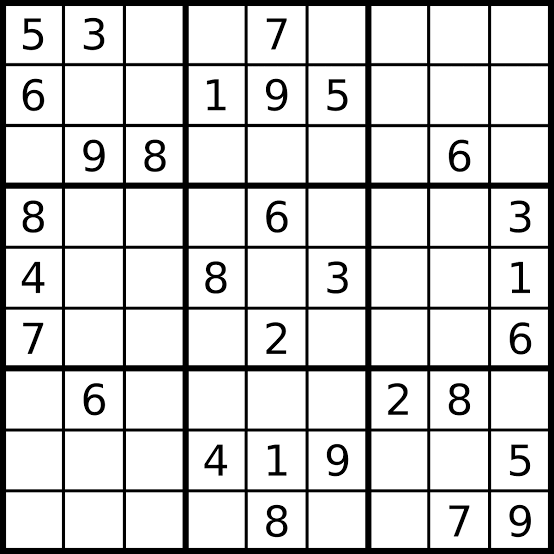
\includegraphics[scale=0.3]{sudoku.png}
  \end{center}
\end{frame}

\begin{frame}
  \frametitle{Sudoku}
  \begin{center}
    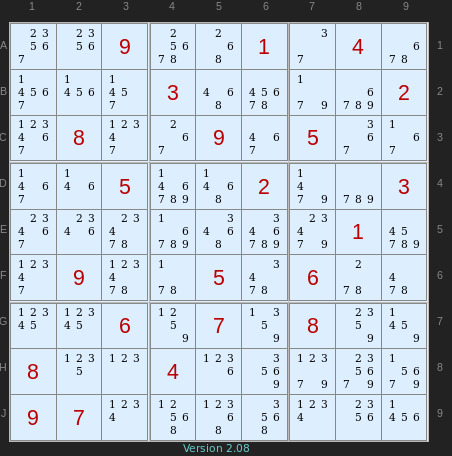
\includegraphics[scale=0.3]{imposible.jpg}
  \end{center}
\end{frame}

\section{Heurística}
\begin{frame}
  \frametitle{Multi-Verse Optimizer}
  \begin{center}
    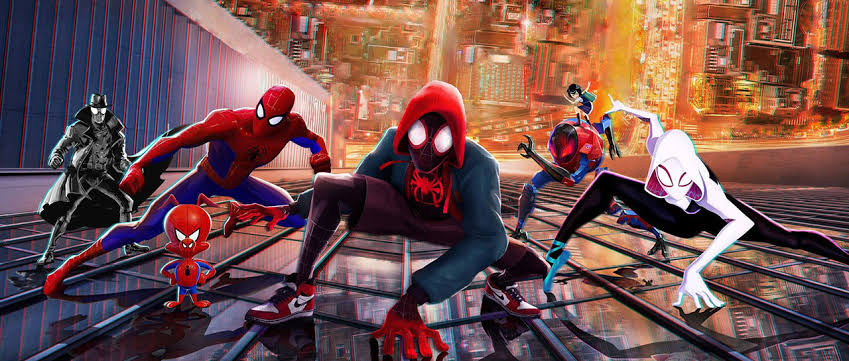
\includegraphics[scale=0.3]{spider-verse.jpg}
  \end{center}
\end{frame}

\begin{frame}
  \frametitle{Multi-Verse Optimizer}
  \begin{center}
    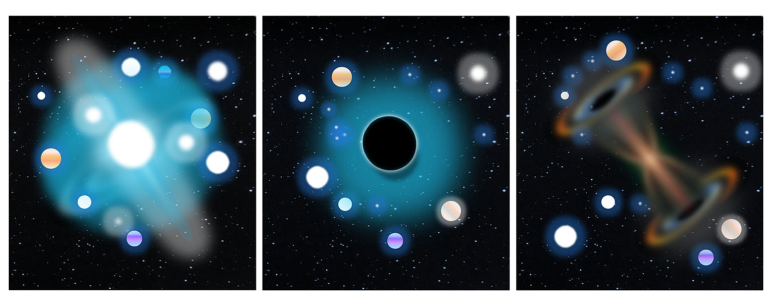
\includegraphics[scale=0.3]{holes.png}
  \end{center}
\end{frame}

\begin{frame}
  \frametitle{Multi-Verse Optimizer}
  \begin{center}
    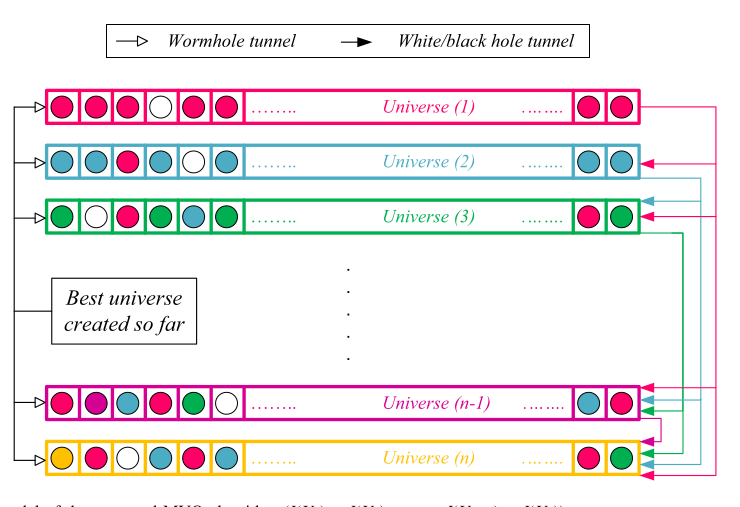
\includegraphics[scale=0.27]{representation.png}
  \end{center}
\end{frame}

\end{document}
